%%%%%%%%%%%%%%%
%%  Template for latex documents
%%  Author: Marco A. Aquino-Lopez
%%  Nota: to get a word document use pandoc
%%  pandoc -f latex Articulo.tex -o Articulo.docx --bibliography=bibliography.bib
%%%%%%%%%%%%%%%%%
%\documentclass [twocolumn,10pt] {article}
\documentclass [10pt] {article}
\usepackage [utf8] {inputenc}
\usepackage[english]{babel}

\usepackage {graphicx}
\usepackage {amsfonts}
\usepackage {amsthm}
\usepackage {amsmath}
\usepackage {natbib}
\usepackage{hyperref}
\usepackage[in]{fullpage} %To have more in the page
%.____         ___________    ____  ___ 
%|    |   _____\__    _______ \   \/  / 
%|    |   \__  \ |    |_/ __ \ \     /  
%|    |___ / __ \|    |\  ___/ /     \  
%|_______ (____  |____| \___  /___/\  \ 
%        \/    \/           \/      \_/ 

\graphicspath{{Figures/}} %Setting the graphicspath

%Extra packages
\usepackage{placeins}

%%%%%%

\date{ }
\usepackage{color}

%%%% To mark notes or added text by Author1 (a1)
%%%% This allows to add notes
%\newcommand{\a1}{\color{red} }  %% begin
%\newcommand{\1a}{ \color{black}} %% end
%\newcommand{\cuta1}[1]{\ac [cut] \ca} %% to mark cut text
%\newcommand{\notea1}[1]{\textcolor{red}{(note)}\footnote{\ac #1 \ca}}  %% To add a note or comment


% %%%% To mark notes or added text by Andres (ac)
% \newcommand{\ac}{\color{red} }  %% begin
% \newcommand{\ca}{\color{black}} %% end
% \newcommand{\cutac}[1]{\ac [cut] \ca} %% to mark cut text
% \newcommand{\noteac}[1]{\textcolor{red}{(note)}\footnote{\ac #1 \ca}}  %% To add a note or comment

% %%%% To mark notes or added text by Marco (ma)
% \newcommand{\ma}{\color{blue} }  %% begin
% \newcommand{\am}{\color{black}} %% end
% \newcommand{\cutma}[1]{\ac [cut] \ca} %% to mark cut text
% \newcommand{\noteam}[1]{\textcolor{red}{(note)}\footnote{\ac #1 \ca}}  %% To add a note or comment


% NOTE: To produce blinded version, replace "0" with "1" below.
\newcommand{\blind}{1}
\newcommand{\papertitle}{
	Evaluation of $^{210}$Pb dating models using simulated datasets
 %A simulation study to compare $^{210}$Pb dating analyses 
}

\begin{document}
	\def\spacingset#1{\renewcommand{\baselinestretch}%
		{#1}\small\normalsize} \spacingset{1}
	%%%%%%%%%%%%%%%%%%%%%%%%%%%%%%%%%%%%%%%%%%%%%%%%%%%%%%%%%%%%%%%%%%%%%%%%%%%%%%
	\if1\blind
	{
		\title{\textbf{\papertitle}}

		\author{Marco A Aquino-L\'opez\thanks{
				Centro de Investigaci\'on en Matem\'aticas (CIMAT),
				Jalisco s/n, Valenciana, 36023 Guanajuato, Gto, Mexico.
				email: \texttt{aquino@cimat.mx} } \thanks{Corresponding author.}
					\and
			Nicole K. Sanderson\thanks{
				GEOTOP Research Centre, Université du Québec à Montréal, 
				Montréal, Québec, H2X 3Y7, Canada. 
				email: \texttt{sanderson.nicole@uqam.ca}}
					\and
			Maarten Blaauw\thanks{School of Natural and Built Environment,
				Queen's University Belfast,
				Belfast, BT7-1NN, UK.
				email:\texttt{maarten.blaauw@qub.ac.uk}  }
					\and
			Joan-Albert Sanchez-Cabeza\thanks{
				Unidad Acad\'emica Mazatl\'an, 
				Instituto de Ciencias del Mar y Limnolog\'ia, 
				Universidad Nacional Aut\'onoma de Mexico, 
				82040 Mazatl\'an, M\'exico.
				email:\texttt{jasanchez@cmarl.unam.mx}} 
					\and
			Ana Carolina Ruiz-Fernandez\thanks{
				Unidad Acad\'emica Mazatl\'an, 
				Instituto de Ciencias del Mar y Limnolog\'ia, 
				Universidad Nacional Aut\'onoma de Mexico, 
				82040 Mazatl\'an, M\'exico.
				email:\texttt{caro@ola.icmyl.unam.mx}} 
					\and
			J Andr\'es Christen\thanks{
				Centro de Investigaci\'on en Matem\'aticas (CIMAT),
				Jalisco s/n, Valenciana, 36023 Guanajuato, Gto, Mexico.
				email: \texttt{jac@cimat.mx}  }
			}
		\maketitle
	} \fi

	\if0\blind
	{
		\bigskip
		\bigskip
		\bigskip
		\begin{center}
			{\LARGE\bf \papertitle}
		\end{center}
		\medskip
	} \fi
\bigskip
\begin{abstract}
The increasing interest in understanding anthropogenic impacts on the environment has led to a considerable number of studies focusing on sedimentary records for the last $\sim$ 100 - 200 years. 
Dating this period is often complicated by the poor resolution and large errors associated with radiocarbon ($^{14}$C) ages, which is the most popular dating technique. 
	To improve chronology resolution for this period, sediment $^{210}$Pb (lead-210) dating is widely used as it provides absolute and continuous dates for the last $\sim$ 100 - 150 years. 
The $^{210}$Pb dating method has traditionally relied on the Constant Rate of Supply (CRS, also known as Constant Flux - CF) model which uses the radioactive decay equation as an age-depth relationship resulting in a restrictive model to approximate dates. 
	In this study, we compare the classical approach to $^{210}$Pb dating (CRS), and its Bayesian alternative (\textit{Plum}). 
To do so, we created simulated depth $^{210}$Pb profiles following three different sedimentation processes, complying with the assumptions imposed by the CRS model, and analysed them using both approaches. 
It is important to note that different laboratories vary in their application of the CRS model.
Results indicate that the CRS model, used in a non-expert mode, does not capture the true age values, even with a high dating resolution of the sediment record, nor does its accuracy improve as more information is available. 
On the other hand, the Bayesian alternative (\textit{Plum}) provides consistently more accurate results even with a relatively small samples size, and its accuracy and precision constantly improve as more information is available.
\end{abstract}
	\noindent%
	{\it Keywords:} Plum, Age-depth models, Chronology, Constant Rate of Supply, Simulations, Comparison.
	\vfill
	\newpage
	\spacingset{1.45} % DON'T change the spacing!

%%%%%%%%%%%%%%%%%%%%%%%%%%%%%%%%%%%%%%%%%%%%%%%%%%%%%%%%%%%%%
%%%%%%%%%%%%%%%%%%%%%%%%%%%%%%%%%%%%%%%%%%%%%%%%%%%%%%%%%%%%%
\section{Introduction}

	Lead-210 ($^{210}$Pb) is a natural radionuclide, part of the $^{238}$U decay chain, which forms in the atmosphere as well as in sediments.
This isotope, with a half-life of 22.23 $\pm$ 0.12 years, is commonly used to date recently accumulated sediments ($<150$ years). 
In recent decades, an increasing number of palaeoecological and pollution studies have focused on these recent sediments \citep[e.g.,][]{Courtney2019} to evaluate human impacts on the environment.
Such environmental studies strongly rely on the accuracy of chronologies to correctly assign dates to geological, chemical, biological and ecological changes.
Unlike other dating techniques such as $^{14}$C (radiocarbon dating), $^{210}$Pb-dating a given single sediment layers is not possible from a single $^{210}$Pb measurement.
Samples are taken along a core (e.g., lake, peatland, marine sediments) at different depths, from which $^{210}$Pb activity is measured.
A $^{210}$Pb-chronology can only be established (1) when a suitable portion of the excess-$^{210}$Pb (atmospheric and/or water column $^{210}$Pb) decay curve is measured, which represents the total inventory of $^{210}$Pb from deposition and runoff, and (2) when certain assumptions about the sedimentation process are met.
%The retrospective enviromental studies strongly rely on the accuracy of chronologies to correctly assign dates to geological, chemical, biological and ecological changes.
That is, unlike other dating techniques, the analysis of a complete series (data set) of $^{210}$Pb measurements must be carried out in order to obtain meaningful dates, see \citet{Aquino2018}.
%Samples are taken at different depths along a sediment core (e.g., lake, peatland, marine sediments) at different depths, from which $^{210}$Pb activity is measured.  
%The whole series of $^{210}$Pb measurements need to be analysed in order to produce a coherent chronology, see \citet{Aquino2018}.


	A range of traditional data analyses, so called ``models'', are available for dating recent sediments using $^{210}$Pb; e.g. the Constant Initial Concentration \citep[CIC,][]{Goldberg1963}, also known as Constant Activity \citep[CA,][]{Robbins1975}, the Constant Flux : Constant sedimentation \citep[CF:CS,][]{Crozaz1964} and the Constant Rate of Supply  \citep[CRS,][]{Appleby1978,Robbins1978,Sanchez-Cabeza2012} also known as the Constant Flux model (CF). 
The main assumption of the CIC model is that sediments have a constant initial $^{210}$Pb concentration. 
Both CF:CS and CRS models assume a constant flux of $^{210}$Pb, but the CF:CS model also assumes that the sedimentation rate is constant. 
The CRS model is by far the most popular (see Figure \ref{fig:210models}) and allows for estimating variable mass accumulation rates.
The flexibility of the CRS model, in terms of its assumptions, comes at the cost of needing to measure a sufficient portion of the excess $^{210}$Pb inventory or the use of interpolation/extrapolation in order to properly estimate the complete inventory of $^{210}$Pb in the sediment. 


\begin{figure}[h!]
	\begin{centering}
		\includegraphics[width=.75\linewidth]{barras.pdf}
		\caption{Frequency of $^{210}$Pb dating models used in papers between 1964 and 2017. Data gathered by \citet{Courtney2019} from a literature review of 271 papers. The models include the CF:CS \citep[Constant Flux - Constant Sedimentation;][]{Robbins1978}, CIC (Constant Initial Concentration) \citep{Goldberg1963,Crozaz1964,Robbins1978} and CRS  \citep[Constant Rate of Supply;][]{Appleby1978,Robbins1978}. }
		\label{fig:210models}
	\end{centering}
\end{figure}

%Caro quiere que este párrafo se integre al párrafo donde se habla de las modificaciones revisar depues  
	The CRS model has undergone several revisions in the last decade in order to improve its applicability and precision. 
There are two types of revisions to this model: (1) revisions to its uncertainty quantification \citep[eg. ][]{Binford1990,Appleby2001,Sanchez-Cabeza2014} and (2) to its application where extra information is available, such as external independent dating markers (e.g. $^{137}$Cs profiles), laminated sediments, tephras, contaminated layers (known sedimentary events) \citep[e.g.][]{Appleby1998,Appleby2001,Appleby2008}. 

	A recent inter-laboratory model comparison experiment \citep{Barsanti2020} presented concerning results when it comes to producing consistent chronologies.
Two measured $^{210}$Pb datasets were sent to 14 laboratories around the world, these laboratories having varying degrees of expertise.
Each laboratory was asked to provide a chronology, given the same data. 
It is important to note that each laboratory applied their preferred model; in most cases the CRS model was used.
This experiment resulted in a wide range of chronologies, independently of the model used, providing different results even when the same model and dataset were used.
The authors reinforced the need to use independent time markers (independent dating sources) to validate and ``anchor" the chronologies, as suggested previously by \citep{Smith2001}.  
This comparison experiment clearly and critically shows the impact that user decisions and applying expert adaptations/revisions have on the resulting chronologies.
In order to replicate and/or update any given chronology, documenting such user decisions becomes extremely important, as is providing raw data; however raw data sets and user decisions are rarely reported.

	Recently, \citet{Aquino2018} presented an alternative to these classical models by introducing \textit{Plum}, a Bayesian approach to $^{210}$Pb dating.
This model treats every data point as originating from a forward model that includes both the sedimentation process and the radioactive decay process.
\textit{Plum} also assumes a constant flux of excess $^{210}$Pb to the sediment, similar to the CRS model (this assumption can be relaxed at the cost of computational power).
Another important difference between the CRS and \textit{Plum} models is that the latter incorporates the supported $^{210}$Pb, which naturally forms in the sediment and is normally treated as a hindrance variable.

	\citet{Blaauw2018} presented a comparison between classical and Bayesian age-depth models construction, both for real and simulated $^{14}$C-dated cores.
They concluded that Bayesian age-depth models provide a more accurate result and more realistic uncertainties under a wide range of scenarios.  
The objective of the present study is to test whether similar results are maintained in a more complex modelling situation, such as the construction of $^{210}$Pb-based age-depth models.
To do so, we compare $^{210}$Pb dates (accuracy) and uncertainties (precision) from the widely applied CRS model against \textit{Plum} using simulated cores, i.e. sedimentation ``scenarios''.
We also aim to observe the learning process of each of the models and estimate the amount of information needed to obtain a reasonable chronology for each model.
This process is of critical importance as the amount of information depends on the number of samples, which in turn depends on the budget, time and user decision of resources allocated to developing the age-depth model. 


%Esto debe ser revisado antes de tener una version final, se esta agregando una sección
	The paper is organized as follows: 
Section 2 provides a short introduction to the most used $^{210}$Pb dating models (CRS, CIC and CF:CS) as well as \textit{Plum}.
Section 3 discussed the consideration and the experimental setup.
Section 4 presents the tools we use for the model comparison, describing the three different sedimentation scenario simulations.
Section 5 compares results for the overall chronologies and for single depths.
Lastly, Section 6 presents the conclusions and discussion of the results obtained in section 5. 

\section{$^{210}$Pb models}

	As previously outlined in Section 1, several methods are used to estimate ages from sediments containing $^{210}$Pb.  
These methods are based on varying assumptions to achieve different chronologies. 
It is important to note that all these models, excluding \textit{Plum}, only deal with unsupported $^{210}$Pb, which is atmospheric $^{210}$Pb -for continental sediments- and/or water column $^{210}$Pb for marine sediments . 
Considering that almost any sediment contains some level of local $^{210}$Pb (i.e., supported $^{210}$Pb), which is constantly replenished, and it is indistinguishable from the excess $^{210}$Pb, the proper estimation of the excess $^{210}$Pb is critical.  
It is important to note that in some cases, users can estimate levels of $^{226}$Ra, which is an extremely useful proxy for estimating the supported $^{210}$Pb, as they are always assumed to be in perfect equilibrium.
In this section, we will describe how each model deals with the supported-excess $^{210}$Pb.

\subsection{Data}

	In order to introduce the nature of the data which these models use to create an age-depth model, we used the data presented by  \citet{Sanchez-Cabeza2012}, in Table \ref{tab:tehuaii}.
This dataset comes from the analysis of $^{210}$Po by alpha-particle spectrometry, which provides measures of $^{210}$Pb, assuming secular equilibrium between both radionuclides. In order to have an estimate of the supported $^{210}$Pb activity, the authors used the deepest 3 samples. When data comes from gamma-ray spectrometry, $^{226}$Ra can be used as a proxy to infer the supported $^{210}$Pb value.  

\begin{table}
\centering
    \begin{tabular}{|c| c| c| c| c| c|}
\hline
	    ID  & Depth ($cm$)  & Density ($\frac{g}{cm^3}$)  & $^{210}$Pb ($\frac{Bq}{kg}$) & sd($^{210}$Pb)  & Thickness ($cm$) \\
\hline
TehuaII-01  & 1  & 1.071583866  & 112.5  & 5.8  & 1\\
TehuaII-02  & 2  & 0.973213378  & 108.4  & 5.7  & 1\\
TehuaII-03  & 3  & 1.121380264  & 102.4  & 5.4  & 1\\
TehuaII-04  & 4  & 1.732484316  & 103.4  & 5.4  & 1\\
TehuaII-05  & 5  & 1.263766643  & 92.9  & 5  & 1\\
TehuaII-06  & 6  & 1.135424096  & 86.6  & 4.8  & 1\\
TehuaII-07  & 7  & 2.085680966  & 70.3  & 3.9  & 1\\
TehuaII-08  & 8  & 1.211092723  & 51  & 3  & 1\\
TehuaII-09  & 9  & 1.339040564  & 45.7  & 2.8  & 1\\
TehuaII-10  & 10  & 2.199381257  & 43.6  & 2.6  & 1\\
TehuaII-11  & 11  & 1.397469527  & 39.7  & 2.4  & 1\\
TehuaII-12  & 12  & 1.280204165  & 34.2  & 2.1  & 1\\
TehuaII-13  & 13  & 1.516059058  & 28  & 1.8  & 1\\
TehuaII-14  & 14  & 1.456445983  & 23.9  & 1.5  & 1\\
TehuaII-15  & 15  & 1.42113905  & 20.5  & 1.4  & 1\\
\hline
\dotfill
TehuaII-16  & 16  & 1.443497137  & 17.1  & 1.3  & 1\\
TehuaII-17  & 17  & 0.451885447  & 14.4  & 1  & 1\\
TehuaII-18  & 18  & 0.630431828  & 15.7  & 1  & 1\\
\hline
    \end{tabular}
	\caption{Data from Tehuantepec Gulf (TEHUAII) reported in \citet{Sanchez-Cabeza2012}. Depth represents the lower depth of each sample section, density is the sample's density which is used to correct for compaction, $^{210}$Pb is the measured $^{210}$Pb in the given sample, sd($^{210}$Pb) is the error reported by the laboratory and thickness is the sample's thickness.  }
	\label{tab:tehuaii}
\end{table}


\subsection{CIC}

The Constant Initial Concentration (CIC) model \citep{Goldberg1963,Crozaz1964,Robbins1978} assumes that the initial concentration of excess $^{210}$Pb at any sediment layer is the same. 
With this assumption, we can define the initial concentration of any layer as $P_0^U = Constant$, by directly using the decay equation the age of any depth as,
\begin{eqnarray}
	t_i = \frac{1}{\lambda}\ln \left( \frac{P_0^U}{P_i^U}\right),
\end{eqnarray}
where $\lambda$ the decay constant of $^{210}$Pb $= 0.03118\pm 0.00017$ yr$^{-1}$), $P_0^U$ and $P_i^U$ are the initial $^{210}$Pb concentration and measured concentration of layer $i$ respectively. 

The main assumption of this model, that sediments have a constant initial $^{210}$Pb concentration irrespective of the sedimentation rate, is particularly strong as it implies that the $^{210}$Pb influx to the sediment surface should be proportional to the mass accumulation. 
This is a very restrictive condition and most likely false for most ecosystems, especially considering the impacts of land use changes on the sedimentation regimes around the world. 
In addition, the CIC model requires the decrease of excess 210Pb monotonically down-core (uncommon in case of variable sedimentation), otherwise, deeper sections with higher concentrations would be younger (age reversal).
As Figure \ref{fig:210models} shows this model is rarely used, and its application is mostly limited to early users or when other models’ requirements are not met.
An example of the use of this model is shown at the end of this section with a comparison to the other models. For details on the application of the model refer to \citet{Sanchez-Cabeza2012}.


\subsection{CF:CS}

This model assumes both a constant initial concentration of $^{210}$Pb at any layer but also a constant accumulation rate over the sediment accumulated mass.  

\begin{eqnarray}
	t_i = -\frac{m_i b}{\lambda},
\end{eqnarray}
where $m_i$ is the accumulated dry mass of the sediment up to layer $i$, and $b$ is approximated using linear regression over the following model,

\begin{eqnarray}
	ln(P_i^U) &= ln(P_0^U) - \frac{\lambda}{r}m_i \\
		   &= \hat{a} + \hat{b}m_i.
\end{eqnarray}

It is important to note that this model is still very restrictive, even if it is more flexible than the previous model. 
In addition, it is even more rarely used in practice, and again, only when the CRS model assumptions are not met.
For the proper implementation of this model, refer to \citet{Sanchez-Cabeza2012}.


\subsection{CRS}

Up to this point, we have dealt with models which have very restrictive assumptions and are simple extensions of the decay equation. 
The CRS \citep{Appleby1978,Appleby1998,Appleby2001,Appleby2008}, in contrast, assumes a constant flux of excess $^{210}$Pb to the sediment and allows for changes in the sedimentation rate. 
In order to allow for flexibility in the sedimentation rate, the CRS model uses remaining activity, obtained by multiplying $^{210}$Pb concentration and the density of the sediment. 

This model also requires that the sediment be measured to the point where excess $^{210}$Pb is not longer detected, i.e., reaching equilibrium or background.
In order to build a chronology, the CRS model uses a ratio between the complete “inventory” (the excess $^{210}$Pb activity accumulated in the sediment column, between the surface and the equilibrium depth, where excess $^{210}$Pb can no longer be detected) and the remaining inventory from depth x to the previously defined equilibrium depth,
\begin{eqnarray}
	t(x)=\frac{1}{\lambda}\log\left( \frac{A_0}{A_x}\right),
\end{eqnarray}
where $A_0$ is the complete inventory, and $A_x$ is the inventory up to depth $x$.


Once more details on the proper use of this and the previous models can be found in \citet{Sanchez-Cabeza2012}.

\subsection{\textit{Plum}}

Lastly, \textit{Plum} is the most recent age depth model \citep{Aquino2018}.
This model is the first Bayesian method for dating $^{210}$Pb sediments and is receiving growing interest from the palaeoecological community, with more applications since its publication than the CF:CS model observed in the literature review by \citet{Courtney2019}.

\textit{Plum} assumes that there exists an (unknown) age-depth function $t(x)$ that relates depth $x$ with calendar age $t(x)$. 
Conditional on $t(x)$, the following model is assumed for the measured $^{210}$Pb ($y_i$) between depths $x_i - \delta$ to $x_i$
\begin{eqnarray}
y_i\mid P^S_i, \Phi_i, \bar{t}\sim \mathcal{N} \left(P^S_i+\frac{\Phi_i}{\lambda} \left( e^{-\lambda t(x_i-\delta)} - e^{-\lambda t(x_i)} \right), (\sigma_i\rho_i)^2 \right). 
\end{eqnarray}
Here $P_i^S$ is the supported $^{210}$Pb in the sample and $\Phi_i$ the flux of excess $^{210}$Pb to the sediment, the age-depth model $t(x)$ is estimated using  a piece-wise linear model constrained by prior information on the sediment accumulation rates  \citep{Blaauw2011}, see \citep{Aquino2018} for details.

This treatment of the data allows for a formal statistical inference on a well-defined model with specific parameters. 
In order to infer the parameters of the model, a Bayesian approach is used.
This differs from the CRS model, which is a not-likelihood based approach to dating.
The CRS model uses the decay equation to obtain an age-depth function, resulting in a more restrictive age-depth model. 
It only deals with the excess $^{210}$Pb, the estimated supported $^{210}$Pb having been previously removed before modelling.
\textit{Plum} has shown to provide accurate results with a realistic precision using different case scenarios \citep{Aquino2018,Aquino2020} - both in simulations as well as for real cores.
Under optimal dating conditions, \textit{Plum} and the CRS model have been shown to provide similar results \citep{Aquino2020}, with \textit{Plum} providing more realistic uncertainties, with minimal user interaction.

\begin{figure}[h!]
 \centering
	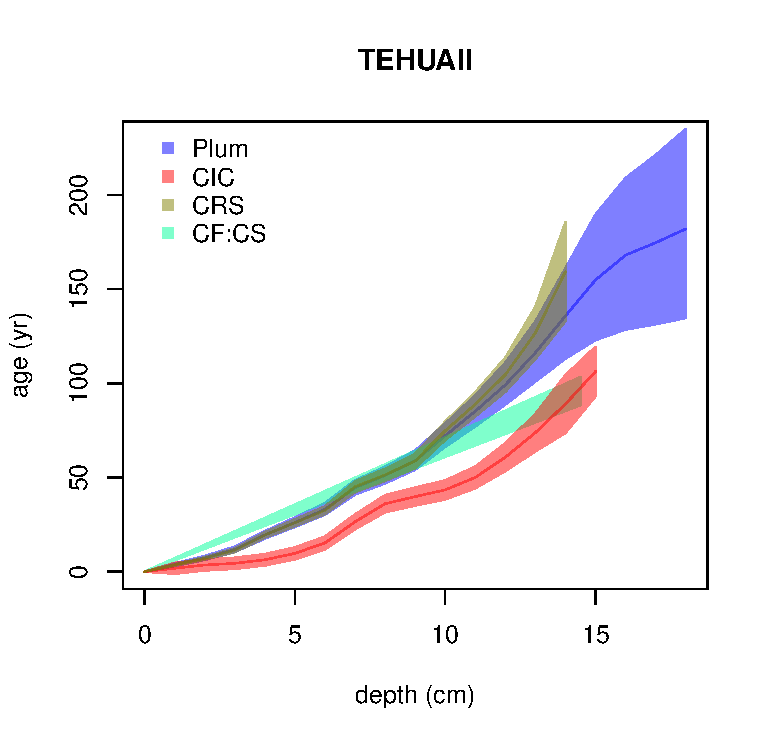
\includegraphics[width=.75\linewidth]{TEHUAII.pdf}
	\caption{Comparison between ages resulting from applying the \textit{Plum}, CIC, CRS and CF:CS models to the dataset in Table 1 and \citet{Sanchez-Cabeza2012}} 
  \label{fig:tehuaii}
\end{figure}

Figure \ref{fig:tehuaii} shows the resulting chronology of each model using the dataset from \citet{Sanchez-Cabeza2012}. 
We observe that the CIC and CF:CS provide very different age-depth models when compared to the CRS and \textit{Plum}. 
As mentioned, the CIC and CF:CS have much more restrictive assumptions which may be the reason to the very different results.
For this reason the main discussion will focus on the CRS and \textit{Plum}.



\section{Model considerations and experiment setup}

Given that the CRS model has had several revisions, the choice of which can considerably affect model outputs as shown by \citet{Barsanti2020}, we decided to apply the original version of the equations provided by \citet{Appleby2001}, with its suggested error propagation calculation; we will call this version of the CRS model the ``classical implementation of the CRS" (CI-CRS). 
We acknowledge that, while this implementation may be less suitable in some particular cases and expert knowledge can greatly improve the precision and accuracy of the model, it will reduce the bias of any particular implementation on our results.

% \subsection{Improvements to the CI-CRS}

Since the late 1970's, when the CRS method was first introduced \citep{Appleby1978,Robbins1978}, the CRS has undergone several improvements.
\citet{Barsanti2020} showed that there exist several modifications and improvements to the CRS, and that the choice of modifications can generate a range of age-depth models.
Some of these improvements rely on independent dates, other isotopes or techniques, and/or require user manipulation to ``force" the method to agree with these independent dates.
One recent improvement, which requires little user manipulation and/or independent dates, is the comprehensive explanation, with expert notes, on the practical used of the CRS model by \citet{Sanchez-Cabeza2012}. 
The same authors presented an improvement to the uncertainty quantification of the age estimates by using the Monte Carlo method \citep{Sanchez-Cabeza2014} and released a publicly available Excel spreadsheet, which facilitates the calculation of their age estimates and Monte Carlo uncertainties. 
Considering that this research focuses on methods with minimal user manipulation, and given that these modifications are laboratory-specific and not made publicly available, we also present and compare results using an R implementation (provided by the authors) of the improved CRS by \citet{Sanchez-Cabeza2014}, here labelled as revised CRS (R-CRS)
% , was used to calculate a chronology of a particular, randomly selected, subsample with 95\% of information and then compared against \textit{Plum} and CI-CRS.
%The goal of this experiment is to quantify the improvement than a particular modification may have on the age estimates provided by the CRS methodology.

% \begin{figure}[h!]
%  \centering
%   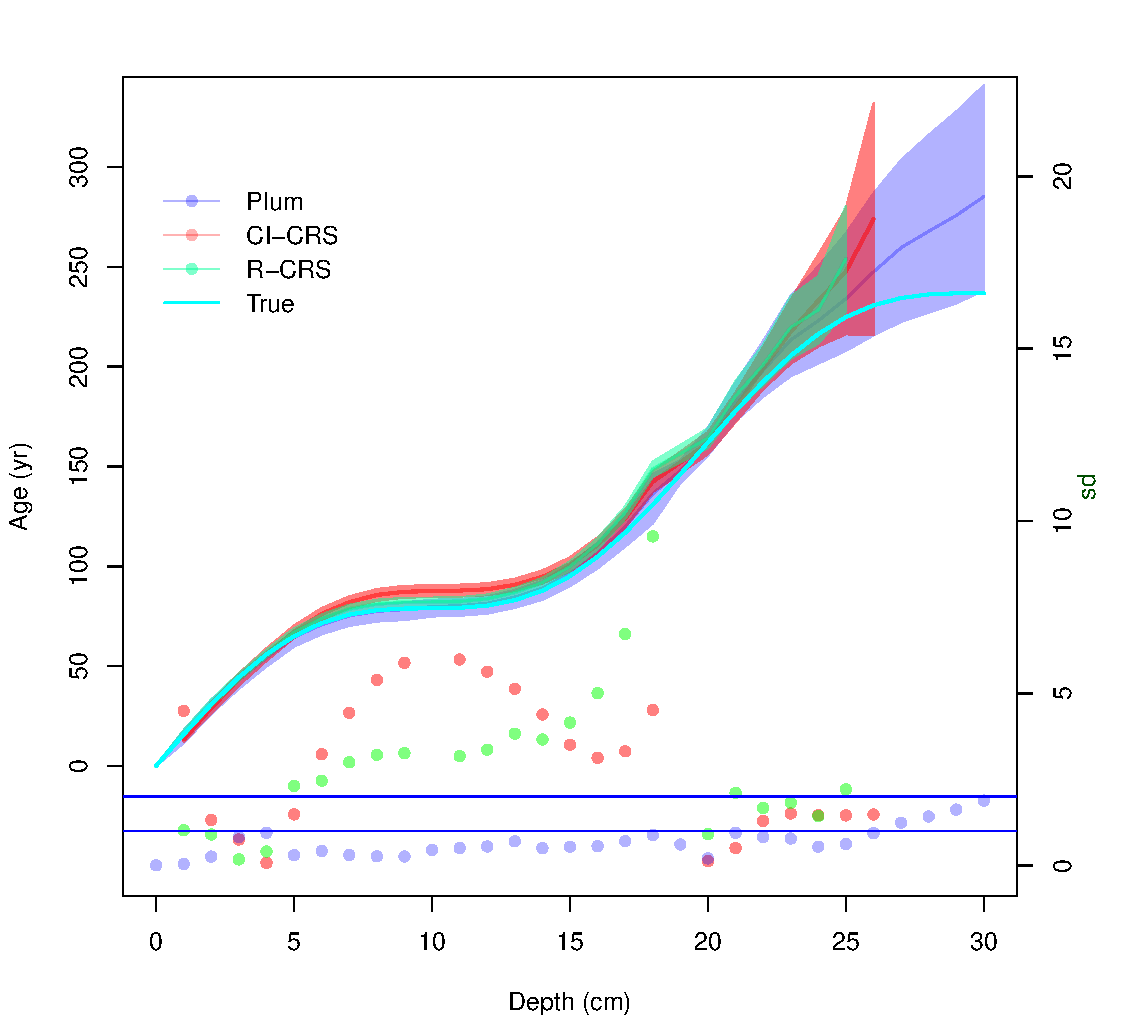
\includegraphics[width=.95\linewidth]{95Comparison.pdf}
% 	\caption{Comparison between the CI-CRS, R-CRS and \textit{Plum}.} 
%   \label{fig:95compa}
% \end{figure}

% Figure \ref{fig:95compa} shows the resulting chronologies for the three methodologies.
% From this figure it is clear that both versions of the CRS model (CI-CRS and R-CRS), with a good percentage of information, are capable of replicating the cyclic changes in accumulation that this scenario presents.
% It is also important to note that the bias of the R-CRS is improved throughout the whole chronology. 
% However, the smaller uncertainties provided by the Monte Carlo method in \citet{Sanchez-Cabeza2014} appear to be the reason that the coverage, of the R-CRS, is larger in some parts of the chronology, when compared to the CI-CRS. 

% The discussion on how large the standard deviation has to be in order to properly represent the uncertainty of the CRS model goes beyond the scope of this research.
% Nevertheless, it is important to point out that the realistic uncertainties provided by \textit{Plum}, are the result of a proper statistical inference where a likelihood is defined.
%% Esto es importante
% In the case of the two version of the CRS model used in this research (CI-CRS and R-CRS) a proper likelihood is never defined and the uncertainties are calculated as a separate part of the model, either by error propagation or the Monte Carlo method.
% This could be the reason that the uncertainty quantification appears to be unrepresentative.

The other models (CIC and CF:CS) were also used in our simulation comparison study, but the results show a considerable bias, as well as an insufficient uncertainties to capture the true age-depth functions, defined in the simulations section, as expected from such restrictive models.
These model runs were performed using the serac R package \citep{Bruel_2020}. 
These results are shown in Appendix A of this paper.





%%%%%%%%%%%%%%%%%%%%%%%%%%%%%%%%%%%%%%%%%%%%%%
%%%%%%%%%%%%%%%%%%%%%%%%%%%%%%%%%%%%%%%%%%%%%%
\section{Simulations (experiment setup)}

	In order to observe the accuracy and precision of any chronology, a known true age-depth function is required.
\citet{Blaauw2018} presented a methodology for simulating radiocarbon dates and their uncertainties, and \citet{Aquino2018} presented an approach for simulating $^{210}$Pb data given an age-depth function $t(x)$.
These simulations follow the equations presented by \cite{Appleby1978, Robbins1978} guaranteeing that the CRS assumptions are met. 
By using the approach presented by \citet{Aquino2018} for simulating $^{210}$Pb data and the structure of uncertainty quantification presented by \citet{Blaauw2018}, reliable simulated $^{210}$Pb data can be obtained.

	This simulation was used to generate three different data sets, that were then sampled. 
Sampling on this datasets mimics the sampling each laboratory, or $^{210}$Pb user, do on a real core. 
The quantity of samples is decided by the resources available to each project (budget, time), as explained by \citet{Blaauw2018}. 
In some cases very few samples are selected to create an age-depth model.

\subsection{Simulation construction}\label{sec:SimConst}

Three different scenarios (see Table \ref{tab:sim_param}) were chosen to simulate sedimentation processes, with their own age-depth functions and parameters. 
These scenarios were selected as they provide three key challenges for the models: 
Scenario 1 presents an age-depth function which is the result of increasing sedimentation and less compaction towards the present (surface), quite common for recent sediments. 
Scenario 2 presents a challenging core structure as the function has a drastic and rapid shift in sediment accumulation around 15 cm depth. Lastly Scenario 3 presents a cyclic and periodic change in accumulation rates. 
Using the age-depth functions and parameters defined in Table \ref{tab:sim_param}, we obtain the $^{210}$Pb activity, or concentration, at any given depth or interval, by integrating the age-depth curve for that interval.  
Although these concentrations may be interpreted as error-free measurements 
(see Figure \ref{fig:true_210}), we replicated the $^{210}$Pb activity uncertainty, following a similar methodology to \citet{Blaauw2018}.
This methodology was chosen as it introduces different sources of uncertainty related to different steps of the measurement process.
Other uncertainty quantification methodologies could be used, but as long as the same methodology and uncertainty are provided to both models the comparison remains valid.
\begin{table}[!h]
	\centering
	\begin{tabular}{l|ccc}
Label    	& 	Age-depth		&	$ \Phi$		& Supported $^{210}$Pb  \\
		&	function $t(x)$		&	($\frac{Bq}{m^2yr }$)	& ($\frac{Bq}{kg}$) 	\\ \hline
Scenario 1 	&	$\frac{x^2}{4} + \frac{x}{2}$	&	100	& 10	\\
Scenario 2 	&	$12x -.2x^2$			&	50	& 25	\\
Scenario 3 	&	$8x+25\sin(\frac{x}{\pi})$	&	500 	& 15		
	\end{tabular}
	\label{tab:sim_param}
	\caption{Simulated age-depth function and parameters used in each scenario}
 \end{table}

\begin{figure}[!h]
 \centering
  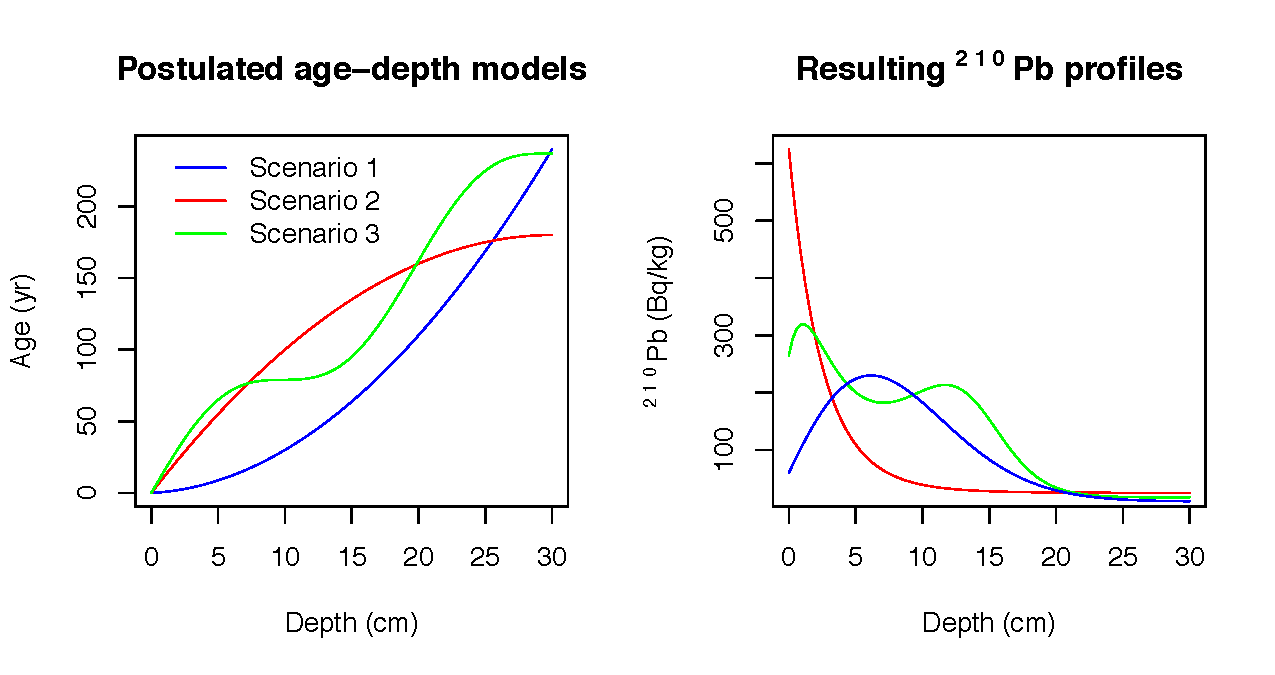
\includegraphics[width=.95\linewidth]{chronology.pdf}
	\caption{Simulated sedimentation scenarios with their corresponding $^{210}$Pb profiles. Left: Age-depth functions for the three different scenarios (Table \ref{tab:sim_param}). Right: Corresponding $^{210}$Pb activity profiles in relation to depth.}
  \label{fig:true_210}
\end{figure}


	Let $C_{\hat{x}}$ be the true $^{210}$Pb concentration in the interval $\hat{x}=[ x-\delta, x)$, given the age-depth function $t(x)$ and parameters $\Phi$ and $A^S$ in each scenario. 
To simulate disturbances in the material, we can introduce scatter centred around the true value, $\theta \sim \mathcal{N}\left(C_{\hat{x}},y^2_{scat}\right)$, where $x^2_{scat}$ is the amount of scatter for this variable (in this case $y^2_{scat}=10$). 
Now, to replicate outliers, a shift from the true value ($X_{shift}$) is defined, which occurs with a probability $p_{out}$ resulting in 
$X_{shift} \sim (1-p_{out}) \delta_0 + p_{out} \mathcal{U}(-x_{shift}, x_{shift})$, where $\delta_0$ is a point-mass at 0.

Finally, to simulate the data provided by the laboratory ($y(\theta')$), we can define as,  
\begin{align}
	y(\theta')\sim\mathcal{N}\left(C_{\hat{x}} + X_{shift}, y^2_{scat} + \sigma^2_{R} \right), 
\end{align}
where $\sigma_R$ is the standard deviation reported by the laboratory. 
$\sigma_R$ is defined as $\sigma_R= \max \left(\sigma_{min}, \mu(\theta')~\varepsilon~y_{scat}~\right)$, where $\sigma_{min}$ is the minimum standard deviation assigned to a measurement. This variable differs between laboratories,we use a default value of $1~ Bq/kg$. 
Finally, $\varepsilon$ is the analytical uncertainty (default 0.01) and $y_{scat}$ an error multiplier (default 1.5).
The default parameters were set in accordance with \citet{Blaauw2018}.


For this study we created a dataset for each simulation by integrating in intervals of $\delta =$1 cm, for depths from  0 to 30 cm, where radioactive equilibrium was guaranteed \citep{Aquino2018}.
The complete simulated $^{210}$Pb data sets can be found in \url{https://github.com/maquinolopez/Paper_Simulations/tree/master/Code/Data}.

\subsection{Model considerations}
In order to create a comparison with minimal user interaction, each model was run automatically, with default settings.
In the case of \textit{Plum}, default settings were used in order to minimize user interaction.
Default settings for \textit{Plum} are; 1 cm bacon sections, 10 $\frac{cm}{yr}$ mean prior accumulation rate, 50 $\frac{yr Bq}{m^2}$ mean prior influx and 10 $\frac{Bq}{kg}$ mean prior supported $^{210}$Pb.
As the CRS model (for both the CI-CRS and R-CRS) assumes that supported and excess $^{210}$Pb have reached equilibrium, in order to reduce user input, we decided to fix the last sample (30 cm depth) for every case, as this allows every model to reach equilibrium.
This step guarantees the consistent application of the CRS model and provides the model with a single bottom-most depth to be removed as required by the CRS model calculation process. 
Furthermore, the CRS model only works with the excess $^{210}$Pb, when certain excess activities reach negative values, the chronology was calculated below that depth.
\textit{Plum} deals with the supported $^{210}$Pb variable automatically, as part of the inference.
Because of this, \textit{Plum}'s resulting chronology always reaches 30 cm, as by default 1 cm sections are used for every simulation.

In the case of the supported $^{210}$Pb and to reduce the influence of this variable in the bias of the models, a constant level of supported $^{210}$Pb was assumed for both models, which coincides with the way in which the simulations were constructed.
For the CRS model, the mean of the supported $^{210}$Pb measurements was calculated and then subtracted from the total $^{210}$Pb to obtain the excess $^{210}$Pb.
This practice differs from some implementations where the $^{226}$Ra is directly subtracted from the total $^{210}$Pb; in this study we decided that in order to reduce the impact single outliers have in the CRS, the mean would provide a much better estimate of this variable.


% In order to provide an objective comparison, the bias of the true age-depth model (in yr), length of the 95\% intervals (in yr) and coverage (bias over the standard deviation) were calculated (the coverage indicates the distance of modelled ages from the true value given the model's own uncertainty). 
% The main discussion will revolve around the coverage as it provide an intuitive measure of the accuracy a model by taking into account the levels of uncertainty provided by each model. 

%%%%%%%%%%%%%%%%%%%%%%%%%%%%%%%%%%%%%%%%%%
%%%%%%%%%%%%%%%%%%%%%%%%%%%%%%%%%%%%%%%%%%
\section{Model comparison}

To allow for a reasonable comparison between models, and to evaluate the effect that varying amounts of information may have on the accuracy and precision of $^{210}$Pb models (reflected in this study as the bias and coverage), the three simulated data sets previously described were used. 
As sample size is strongly dependent on project's budget and time, samples from the entire core or a portion of the core could be measured or only a portion of it.
In order to analyzed the effects of this parameter, samples of size $m$ were randomly generated provided a percentage of information, e.g., for a 20\% information a dataset with 6 random 1-cm samples -out of a possible total 30 1-cm samples- is created.
This sample was then used to create the chronology and calculate the bias, length of interval and coverage:
100 of these sub-datasets were created for different information percentages (from 10\% to 95\% at 5\% intervals - i.e., 10\%, 15\%, 20\%,...,95\%). 
The complete dataset was also used (i.e., 100\% information percentage sample, or fully analyzed core).
Once a dataset was created, the CRS model and \textit{Plum} were applied (CIC and CF:CS were also applied and results are shown in the appendix).  
Both sets of outputs were then compared against the true known age value, see Figure \ref{fig:comparison1r}.

\begin{figure}[!]
	\centering
	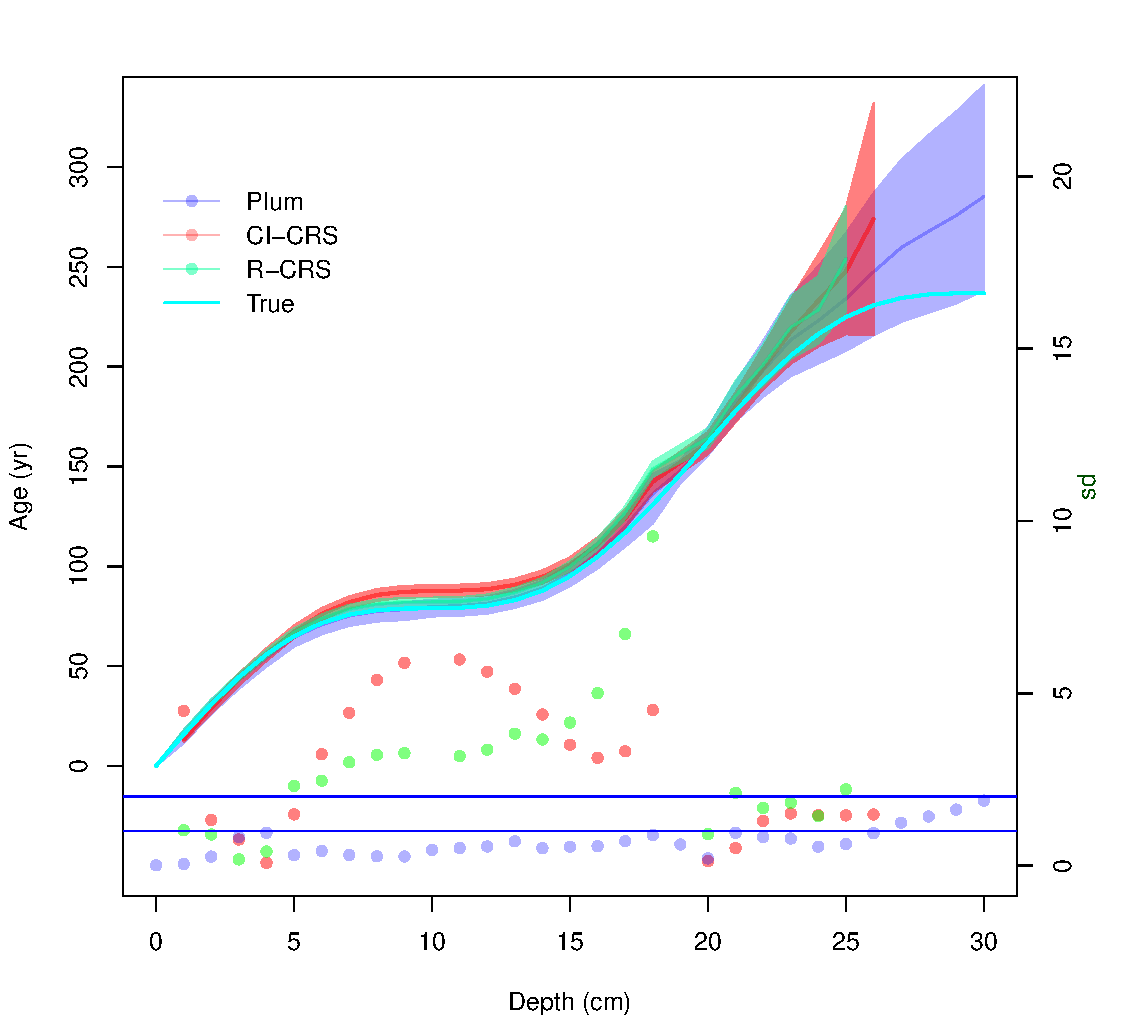
\includegraphics[width=\linewidth]{95Comparison.pdf}
		\caption{Comparison between \textit{Plum}, R-CRS and CI-CRS model against the true age-depth model using 95\% of the information percentage (using 1-cm samples). Lines show the age estimates with the 95\% credible intervals (\textit{Plum}) and the 95\% confidence interval (CI-CRS). Dots show the coverage, i.e. the distance between the inferred age and the true age in relation to the standard error (the standard deviation in the case of the CI-CRS and the length of the confidence interval divided by 4 in the case of \textit{Plum}). The vertical right-hand axis shows how many standard deviations each model is from from the true age.  }
		\label{fig:comparison1r}
\end{figure}

Figure \ref{fig:comparison1r} shows a single ``snapshot", as an example of the comparison between the $^{210}$Pb models against the true value. 
As we are dealing with a total of $n =$ 5333 simulations, in order to evaluate the overall precision and accuracy of both models, we decided to calculate the mean bias of the true age-depth model (in yr), the mean of length of the 95\% intervals (in yr), as well as the mean coverage indicating the distance of modelled ages from the true value given the model's own uncertainty at each depth.  

\begin{figure}[!]
 \centering
  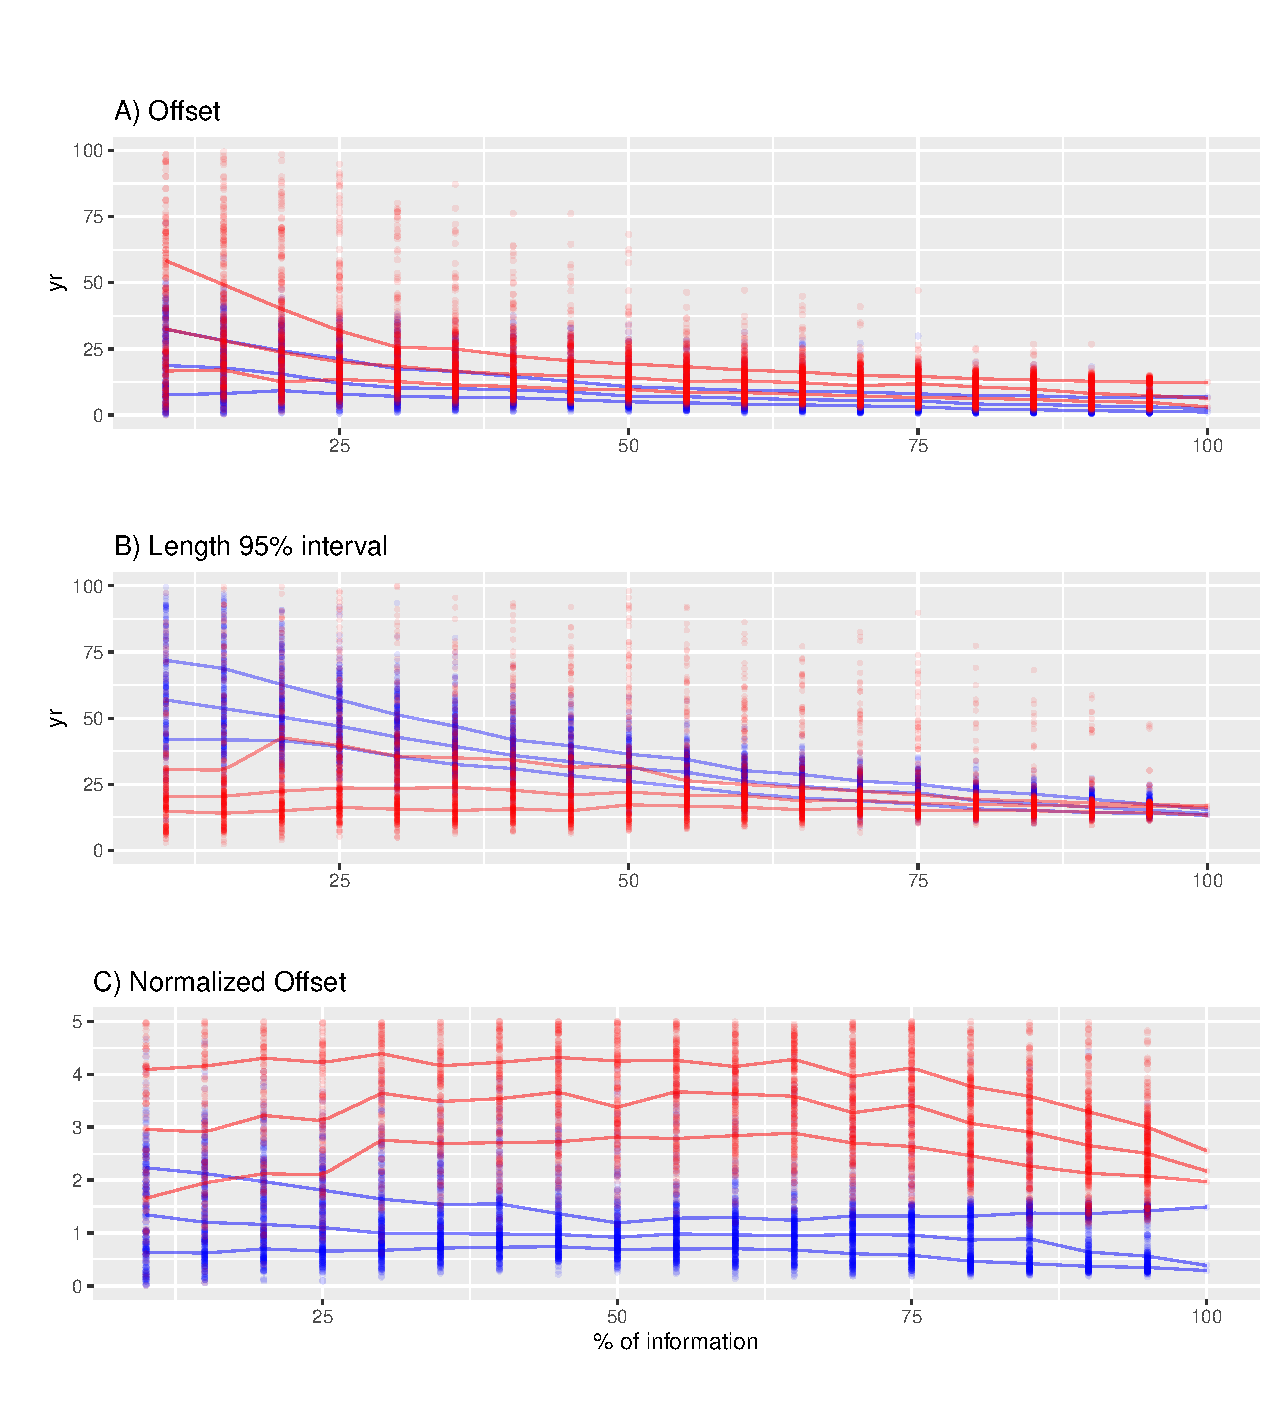
\includegraphics[width=.75\linewidth]{AccPrec.pdf}
	\caption{Top panel A) shows the bias between the modelled and true age of the CI-CRS (red), R-CRS (green) and \textit{Plum} (blue). This panel shows how \textit{Plum} provides a small bias in almost every scenario with both models improving their bias as more information is available. Middle panel B) shows the 95\% confidence intervals and credible intervals in the case of \textit{Plum}. It is clear, from this panel, than the uncertainty provided by \textit{Plum} is a significantly bigger for low percentages of information and it constantly improves as more data is available, whereas the lengths of the intervals provided by the CI-CRS and R-CRS appear to stay constant regardless of the available information. Bottom panel C) shows the coverage, presenting the distance between the modelled age and the true age divided by the standard deviation (in the case of \textit{Plum}, the length of the 95\% interval divided by 4). This panel shows that the CI-CRS and R-CRS model's calculated standard deviation (on average) is incapable of capturing the true age. On the other hand, \textit{Plum}'s credible intervals almost always capture the true age even when little information is available.}
  \label{fig:accpre}
\end{figure}


Figure \ref{fig:accpre} shows similar results to those presented by \citet{Blaauw2018}. 
The classical model (CI-CRS and R-CRS) at first appears to provide a similar results (similar biasses) to the Bayesian alternative (\textit{Plum}), but at higher estimated precision, if we only consider the length of the 95\% interval. 
It is important to note that the CI-CRS and R-CRS models' biases do improves with more information is available.
However, if we do not consider the effects of both the bias and length of the interval together, the results are not favourable to the CI-CRS. 
To have a more realistic representation of how the models capture the true age-depth relationship, we consider the coverage. 
This variable shows the degree to which the average models contain the truth within their uncertainty intervals (normalized to one standard deviation). 
Any model with a coverage larger than two (two standard deviations) is incapable of capturing the true ages within its uncertainty intervals.  
This means that, while the CI-CRS and R-CRS estimate smaller uncertainties and the ages improve as sample size increases, it does so at the cost of accuracy as the improvements are not sufficient to capture the true age.
It also appears that the length of the 95\% interval and bias are not affected by how much information is provided to the CRS model.

On the other hand, \textit{Plum} seems to provide increasingly accurate results as more information is added to the model.
This again coincides with the results outlined by \citet{Blaauw2018}. 
When we observe the regular bias (not normalized), we find that \textit{Plum} provides a smaller bias in comparison to the CI-CRS and R-CRS models; this, in combination with slightly larger (more realistic) modelled uncertainties, results in more consistently accurate age-depth models that are capable of capturing the true values within their uncertainty intervals. 
This result supports the claim that \textit{Plum} provides more realistic uncertainties compared those obtained by the CI-CRS and R-CRS. 
Another important statistic to take into account is that 87.86\% (4686/5333) of \textit{Plum}'s runs remain within the 2 standard deviations, opposed to 7.48\% (399/5333) of the CI-CRS models runs. 
Furthermore, only 0.54\% (29/5333) of the CI-CRS models runs remain under one standard deviation, which is the most commonly reported interval when reporting CI-CRS results, with R-CRS providing very similar results.
We also observe that \textit{Plum} increases its accuracy and precision to produce a better chronology as more information is available, whereas the CI-CRS and R-CRS models do not improve their coverage with additional data. 
As we obtained very similar results from both the CI-CRS and R-CRS, the discussion will now focus on the CRS in general taking the CI-CRS as its base for the following calculations.

In order to evaluate whether certain models are better predicting ages at certain section of the sediment cores, we look at the coverage of every depth. 
These results are valid for the overall chronology (mean bias, interval and coverage of the overall chronology). 

\begin{figure}[!]
	\begin{centering}
		\includegraphics[width=\linewidth]{depthsnew.pdf}
		\caption{Coverage of every sample at every depth for the three simulated scenarios - CI-CRS age estimates at sample depths and \textit{Plum}'s age estimates at 1 cm intervals. Dots go from lowest information percentage samples (few dated depths; red) to high percentage samples (nearly completely dated cores; purple). The CI-CRS's coverage shows no learning pattern at any particular depth regardless of the available information. This means that the model can provide a reasonable chronology with low levels of information or a very inaccurate age estimate with high levels of information at any given depth resulting in an unrealistic age-depth model. On the other hand, \textit{Plum} demonstrates a systematic improvement in its age estimates as more data is available. These results support that a Bayesian approach can consistently provide more reliable results.     }
		\label{fig:depths}
	\end{centering}
\end{figure}

Figure \ref{fig:depths} shows the coverage of every simulation according to depth for both models.
\textit{Plum} shows a clear learning structure which depends on the information available to the model.
The information percentage appears to be irrelevant to the coverage of the CI-CRS model, contrary to the results obtained by \textit{Plum}.
It is important to note that the inaccuracies of the CI-CRS model are not exclusive to any particular sections of the chronology; this is most likely driven by the small uncertainties estimated by the CI-CRS model.
%See below for a discussion of how \textit{Plum} behaved in sedimentation simulation 2.   



%%%%%%%%%%%%%%%%%%%%%%%%%%%%%%%%%%%%%%%%%%
%%%%%%%%%%%%%%%%%%%%%%%%%%%%%%%%%%%%%%%%%%
\section{Discussion and Conclusions}

This research focuses on exploring the uncertainty and precision of the most commonly used $^{210}$Pb dating methods (CRS, CIC and CF:CS) in contrast to the Bayesian alternative (\textit{Plum}).
By using different scenarios, three different simulations were created.
These simulations were then sub-sampled at different percentages of information in order to observe the effects that different sample sizes have on the resulting chronology. 
This experiment provided an objective comparison of the accuracy and precision of both methods.

The experiment was conducted on two levels.
First, we evaluated the overall accuracy and precision of the method.
The mean of the bias, length of the 95\% confidence and credible intervals, as well as the coverage were measured.
Second, we quantified the ability of each model to capture the true value in their credible/confidence interval, and the coverage of each scenario according to depth. 
These two comparisons provided a good picture of the difference in precision and accuracy between these methods.

From the overall accuracy (see Figure \ref{fig:accpre}) it is clear that both the CRS model and \textit{Plum} reduce their bias as more data becomes available, with the Bayesian method providing, on average, a smaller bias regardless of the sample size. 
In terms of precision, the Bayesian method is providing much larger uncertainties when small sample sizes are used. 
It is only with 60\%, or more of information that the length of the intervals becomes comparable. 
This is a consequence of the linear/exponential interpolation between data points used by the CRS method, in contrast to the Bayesian approach (\textit{Plum}).  
As has been previously discussed by \citet{Aquino2020}, the larger uncertainties provided by \textit{Plum} are more realistic, as confirmed in this work.
Further evidence that these uncertainties are more reasonable is that the length of the credible intervals becomes smaller as more data becomes available. 
On the other hand, the length of the confidence intervals provided by the classical model (CRS) remain almost constant at any sample size.
Lastly, the coverage, which shows the ability of the model to capture the true values within their intervals, shows that the classical model (CRS) on average is incapable of capturing the true values within its 95\% confidence interval. 
These results are concerning, considering that the $^{210}$Pb dating community rarely report 95\% confidence intervals and instead tend to use only 65\% confidence intervals (one standard deviation intervals).
On the other hand, \textit{Plum}'s coverages always remain $\leq 2$, therefore guaranteeing that on average the true value is captured within its 95\% credible intervals, even with small sample sizes.
\textit{Plum}'s coverages are constantly improving and reaching stability with 50\% or more, of information percentage.
These experiments show that the Bayesian method, on average, provides more reliable results, for both precision and accuracy, no matter the amount of information.


As the coverage shows the ability of each model to capture the true value within its intervals, this variable can be used to evaluate whether any given method is better at estimating certain time period.
Figure \ref{fig:depths} presents the performance of both the CRS model and \textit{Plum} for every simulated scenario.
It appears that the coverage of many of the CRS chronologies are $> 2$ throughout the whole chronology, meaning that the model does not have a period of time for which it is more precise. 
Moreover, the CRS, as applied, does not exhibit a clear learning pattern, where the coverage appears to be indifferent to the amount of information available.
It appears that even high levels of information percentage provide coverages $> 2$, in some cases closer to 4 for scenarios 2 and 3.
\textit{Plum} on the other hand, shows a structure where more data is reflected in improved models in scenarios 1 and 3.
It is only at low levels of information where \textit{Plum}'s coverage is $>2$.
Scenario 2, on the other hand, presents a case where \textit{Plum} is both incapable of capturing the true value, for depths $>15$ cm, and it appears that as more data becomes available the model provides worse results. 
This may be of concern if we do not recognized that this scenario is unrealistic as it presents an extreme change in the accumulation around 15 cm, which coincides with the depth at which the coverage becomes $>2$.
However, it is also important to acknowledge that this experiment was performed using default settings.  
In a real-world scenario the user typically has some prior knowledge of the sedimentation process, about the site of interest, which could be incorporated as prior information to the model to improve the resulting chronology for both the CRS and \textit{Plum} models.

% The results obtained by this experiment appear to persist even in the case of the revised version of the CRS model (R-CRS).
% The R-CRS model appears to improve the bias but this improvement appears to be nullified by the smaller uncertainties presented by \citet{Sanchez-Cabeza2014}.
% The question of which version of the CRS provides the best result is beyond the scope of this research and is dependent on expert application of the model.
% Nevertheless, it is important to note that that the bias, related to the CI-CRS and R-CRS, are reasonably small at certain sections of the sediment, but the uncertainty quantification of both methods is overly optimistic.  

In conclusion, the use of the Bayesian age-depth models is preferred for the consistent construction of sediment chronologies, not only on radiocarbon-based chronologies as presented by \citet{Blaauw2018} but also in the more complex case of $^{210}$Pb shown here.
While the classical approach provides reasonable results regarding the bias, the uncertainty quantification in these methods needs improvement as it does not rely on a proper statistical structure. 
In a real-world scenario, it is impossible to measure the true bias of a method and therefore a proper uncertainty quantification becomes extremely important.
These results support the recommendations presented by \citet{Smith2001,Barsanti2020} where the CRS method, or any dating methodology, should be validated using independent dating markers. 

Lastly, it is important to highlight the benefits of the Bayesian methods.
From both \citet{Blaauw2018} and the present work, it is shown that Bayesian methods constantly improve as more data are added, the uncertainty associated to the method is realistic and coherent with the amount of information available. 
This leads to chronologies that are capable of capturing the true age in their credible intervals, especially with minimal expert input (unlike the CRS which relies on expert modifications). 
The ability to capture the true value in the credible intervals becomes important when the problem is associated with decision making processes, as it provides a more realistic picture of the available knowledge of the process. 
Given that $^{210}$Pb-dating is now widely-used in pollution, environmental and climate change studies, which potentially have a high impact on both policy-making and public perception, realistic age estimates and uncertainties become extremely important.

\section{Acknowledgments}

The authors are partially funded by CONACYT CB-2016-01-284451 and COVID19 312772 grants and a RDCOMM grant.
The corresponding author is funded by CONACYT through the postdoctoral residence program with CVU  489201.


\bibliographystyle{apalike}
\bibliography{bibliography.bib}
\newpage




\section{Supplementary Material}
\label{sec:supp_mat}
Data for each simulation and code used are hosted at: \url{https://github.com/maquinolopez/Paper_Simulations}

\section{Appendix A}

Bias, length of 95\% confidence intervals (credible intervals for \textit{Plum}) and coverage of the CIC and CF:CS models are shown in Figure \ref{fig:CIC-CFCS}.
As can be observed and as expected the bias of the CIC model (which can be considered the simplest model) is much bigger when compared to any other alternative and it does not decrease as more data is available.
The confidence interval remains regardless of the information available, and coverage is almost always above two, which means that the uncertainties are not sufficient to capture the true age-depth model.
On the other hand the CF:CS model does decrease its bias as more data is available and after 60\% to 70\% this decrease does not seen improve.
The length of the interval remains the same regardless of the information available and the coverage just like the CIC model is almost always above 2 meaning that the uncertainties are not sufficient.

These results are consistent with the discussion in the paper as classical model appear to not improve as more data is available. Its bias does decrease as more data is available (in the case of the CF:CS model) but its uncertainty is underestimated which in turn does not allow the method to have a reasonable coverage. 


\begin{figure}
	\begin{centering}
		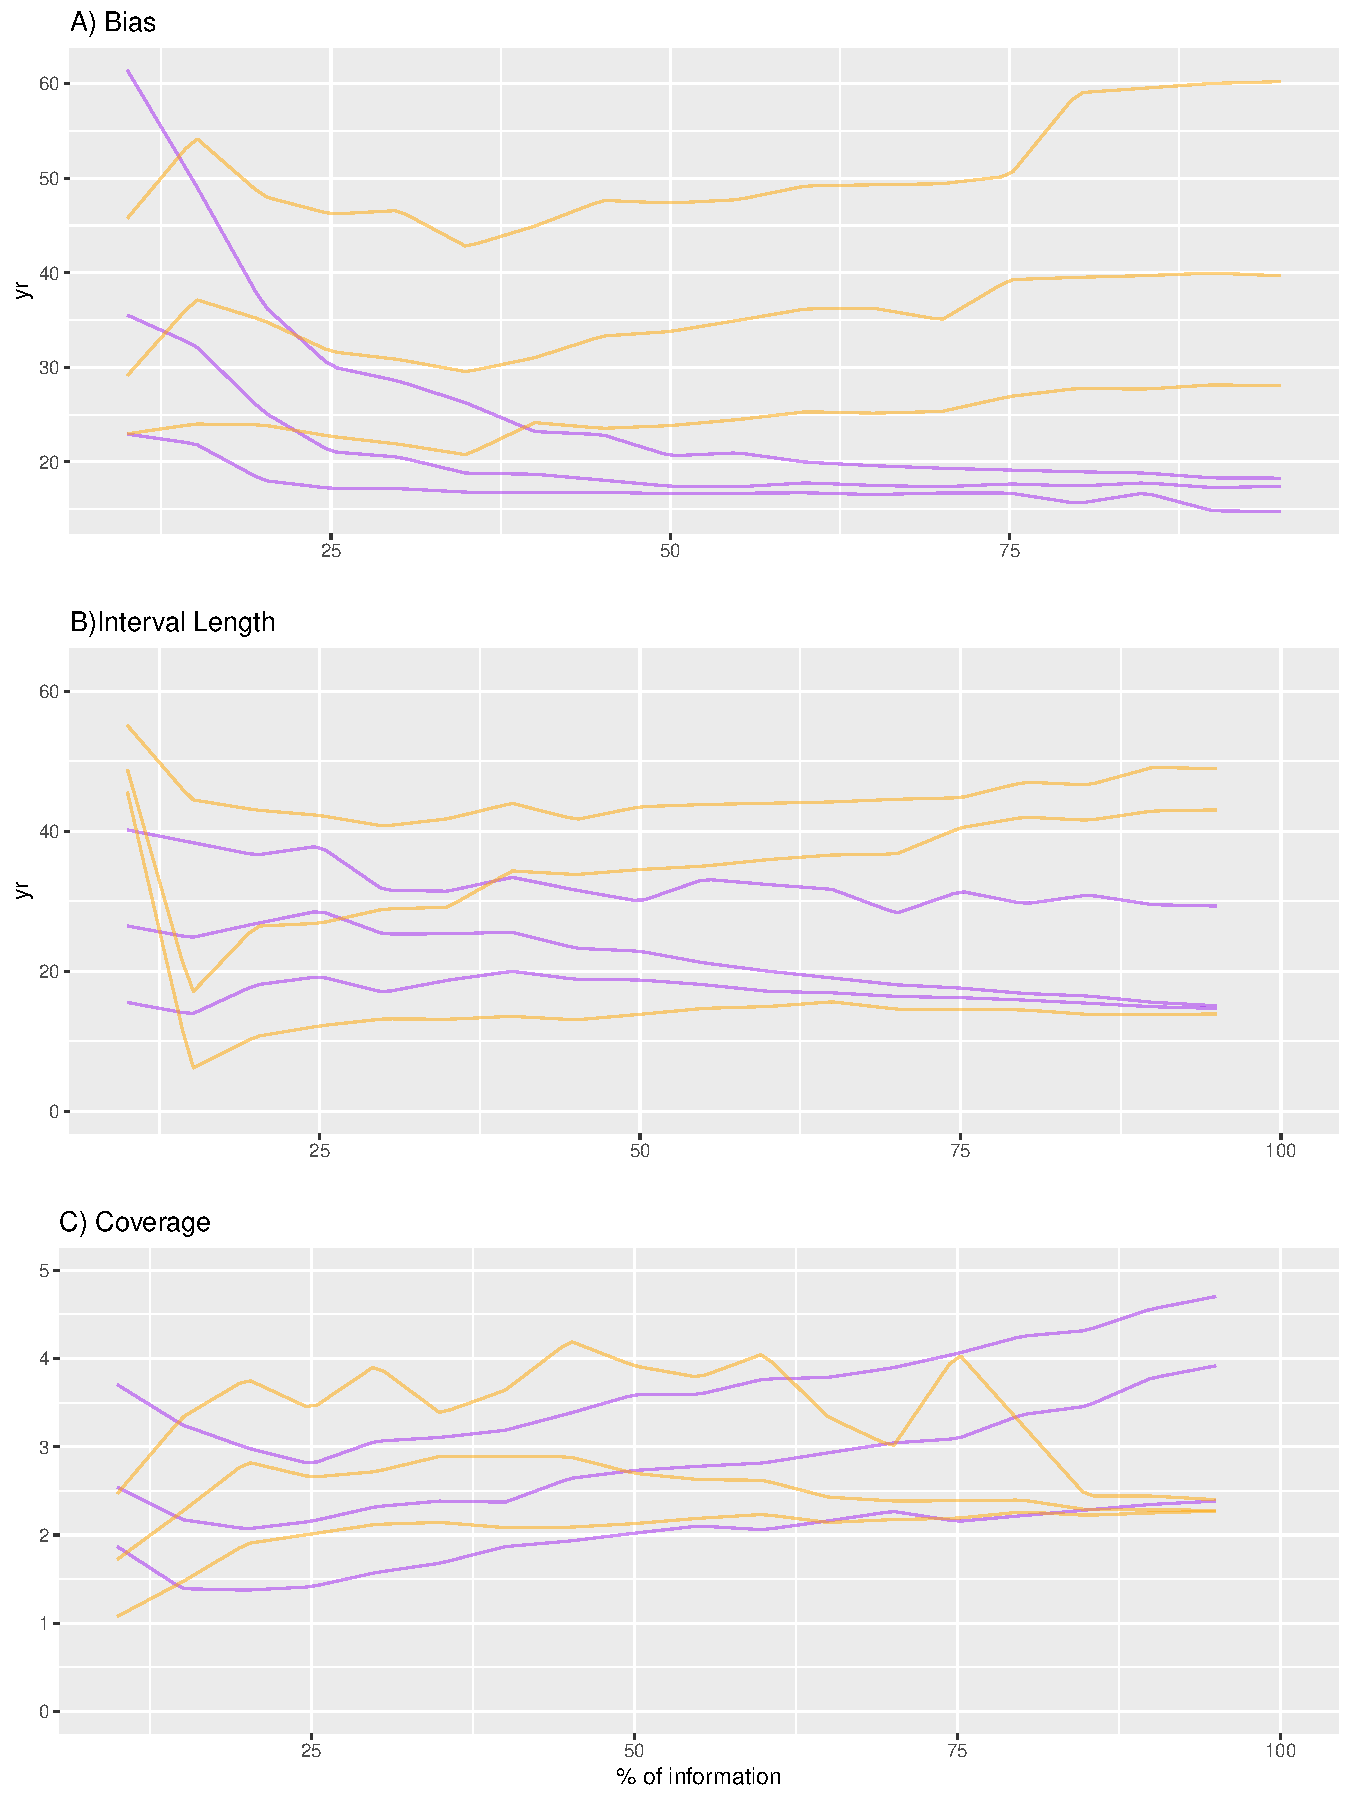
\includegraphics[width = 13cm]{AccPrec-appendix.pdf}
		\caption{ Top panel A) shows the bias between the modelled and true age of the CF:CS (purple) and CIC (Orange). Middle panel B) shows the 95\% confidence intervals (credible intervals for \textit{Plum}). Bottom panel C) shows the coverage, presenting the distance between the modelled age and the true age divided by the standard deviation. }
		\label{fig:CIC-CFCS}
	\end{centering}
\end{figure}

\end{document}
